\documentclass[a4paper,12pt]{report}

\usepackage[english]{babel}
\usepackage{blindtext}
\usepackage{microtype}
\usepackage{graphicx}
\usepackage{wrapfig}
\usepackage{enumitem}
\usepackage{lscape}
\usepackage{amssymb}
\usepackage{epstopdf}
\usepackage{algorithm}
\usepackage{algorithmic}
\usepackage{subfig}
\usepackage{float}
\usepackage{wrapfig}
\usepackage{fancyhdr}
\usepackage{amsmath}
\usepackage{index}
\usepackage{float}
\usepackage{titlesec}
\usepackage{cite}
\usepackage{relsize}
\usepackage{pdflscape}
\usepackage{cite}
\usepackage{geometry}
\usepackage{afterpage}
\usepackage[parfill]{parskip}
\usepackage{hyperref}
\setlength{\footskip}{45pt}
\setcounter{secnumdepth}{3}
\newcommand{\R}{\mathbb{R}}

\graphicspath{ {./images/} }
\hypersetup{
    colorlinks,
    citecolor=black,
    filecolor=black,
    linkcolor=black,
    urlcolor=black
}

\title{\Huge{\textbf{Improving the Reliability of Artificial Intelligence}}\\
\vspace*{0.3cm}
\Large{Capstone Report}}

\titleformat{\chapter}[display]
    {\normalfont\bfseries}{}{0pt}{\huge}\author{Ajal Singh - 12621189\\
    Supervisor: Diep Nguyen}
\date{\today}

\begin{document}
\maketitle
\tableofcontents
    \thispagestyle{empty}
\listoffigures
    \thispagestyle{empty}
\listoftables
    \thispagestyle{empty}


%% Engineering Research Problem
\chapter{Engineering Research Problem}
\setcounter{page}{1}
\label{chap:chap1}

\section{Background }
As the use of Artificial Intelligence (AI) and Machine 
Learning (ML) continues to grow throughout the world 
in high-risk applications, models have become 
ever-increasingly complex and diverse. As a result, 
they often become prone to accidents where unintended 
and harmful behaviour is observed, and consequently are 
scrutinized as disruptive and unreliable solutions. The 
recent emergence in smart cities have seen AI and ML being 
used in various applications such as transportation, 
healthcare, environmental, and public safety as depicted in Figure 1.1.

\begin{figure}[h]
    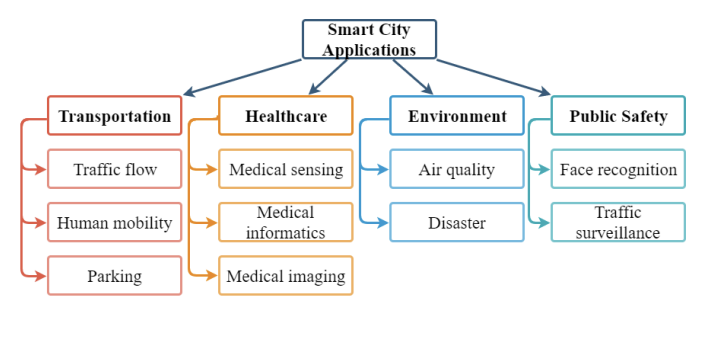
\includegraphics{smart_city_applications.png}
    \caption{Smart City Artificial Intelligence Applications \cite{chen}}
    \label{fig:smart}
\end{figure}

\enlargethispage{2\baselineskip}
For an AI/ML system to be considered reliable, it must 
perform tasks when required as it was originally 
intended, produce consistent results using real-world 
data (and shifts in data), and remain robust and 
predictable. This means it must also fail in a 
predictable manner \cite{Saif}. 

\section{Applications}
One of the most discussed and disruptive applications of ML is facial 
recognition systems used by authorities which fails to distinguish 
between darker skin individuals. This technology is used to assist the 
police in identifying potential criminals/suspects and often leads to 
wrongful arrests of dark-skinned people \cite{Moutafis}. This example highlights the 
importance and the need for reliability in ML solutions. 

There are many more applications where reliability is crucial due to the 
potential consequences. Cancer diagnosis systems trialled in the US are 
failing to detect cancer in patients in differing hospitals and/or countries which may result 
in death. As another example, unintended behaviours in traffic management systems would 
increase congestion resulting in poor ambient air quality and noise 
pollution.

The rapid technological changes in manufacturing have produced a boom 
in Industry 4.0 applications involving Artificial Intelligence, connected
 devices (IoT) and Big Data. A paper on use cases of AI in Industry 4.0 
 summarises the advantages ML, \textit{“AI with machine learning technique can 
 automate the manufacturing process which increase the productivity, 
 efficiency, optimize production cost and reduce manual error” }\cite{9004327}. A 
 key area is predictive maintenance where real-time equipment data is 
 captured and historical equipment data is evaluated using AI and ML 
 models to estimate the equipment life cycle and hence perform timely 
 maintenance to reduce or eliminate down-time. Down-time is undesirable
for manufacturers as it equates to the loss of revenue.

AI in cybersecurity helps protect enterprises by detecting unusual 
activity, patterns, and malicious behaviour and can respond to different 
situations. For manufacturers, this could be used for asset protection 
while banks and financial institutions may use this form ML to detect suspicious 
activity and fraud \cite{9004327}. 

\section{Project Contextualisation}
A tutorial presented by Suchi Saria and Adarsh Subbaswamy of John Hopkins University \cite{saria2019tutorial} postulates some causes and failure prevention techniques for use in supervised learning systems (regression and classification). 
Some of the sources of unreliability discussed are the use of inadequate data, changes in training and deployment environments, and model misspecification. 
These aforementioned causes will form the basis of this research project.

\enlargethispage{-\baselineskip}
Another reliability issue is discussed in a separate paper, \textit{‘Concrete Problems in AI Safety’} \cite{Amodei} is the prevalence of reward hacking in Reinforcement Learning systems. 
Reward hacking is the AI agent’s ability to cheat the system to achieve the highest reward in an unintended way. 
For example, a positive reward may be given to a traffic management system when there is no congestion. However, the AI model decides to divert all traffic through alternative routes essentially shutting down this particular road/intersection. 
This prevents congestion but does not perform as desired. This notion is also investigated in this research project.

\section{Research Question}
\noindent\rule{\linewidth}{0.4pt}
\begin{quotation}
\textit{How can the reliability of Artificial Intelligence be improved against 
inadequate data labelling, unsuitable algorithm choices, and reward 
hacking?}
\end{quotation}
\noindent\rule{\linewidth}{0.4pt}

%% Methodology
\chapter{Methodology}
This project has been divided into three main sections based on the factors of unreliability mentioned earlier in \hyperref[chap:chap1]{Section 1}. 
The main factors studied in this project are:
\begin{itemize}
    \item Label Bias and Environmental Datashift
    \item Suitable Algorithm Selection
    \item Reward Hacking
\end{itemize}

\section{Label Bias and Environmental Datashift}
To investigate the effect of biased data labelling we will train two models using a single independent algorithm. 
One will use biased data while the other uses unbiased data. 
These datasets will be modelled using the mathematical framework outlined in the conference paper \textit{‘Identifying and Correcting Label Bias in Machine Learning’} \cite{Jiang}. 
Each model will be trained and evaluated using data which has been split from the same distribution. 
For a model to be considered reliable it must be able to properly generalise or adapt well to new and unseen data. 
A good, reliable model can achieve high accuracy scores with low variance between datasets. 
Therefore, both of these trained models will then be fed previously unseen data (i.e. deployment data) to determine its ability to generalize.

\section{Suitable Algorithm Selection}
As can be seen in Figure 2.1, when it comes to AI and ML, the appropriacy of solutions or algorithms depends on elements such as the specific application and the level of supervision required. 
More often than not, more than one algorithm could be a viable solution (see \hyperref[fig:algor]{Figure 2.2}). 
Therefore, to investigate suitable algorithm selections, models will be trained with a single dataset using different algorithms (with different assumptions). 
They will then be tested for accuracy to determine suitable algorithm choices. Evaluating the reliability of a model is dependant of the model type. 
Accuracy, precision and recall are three common metrics we can use to evaluate a model. 
However, depending on certain applications, other complex means of metric evaluation may be necessary. 

\begin{figure}[h]
    \centering
    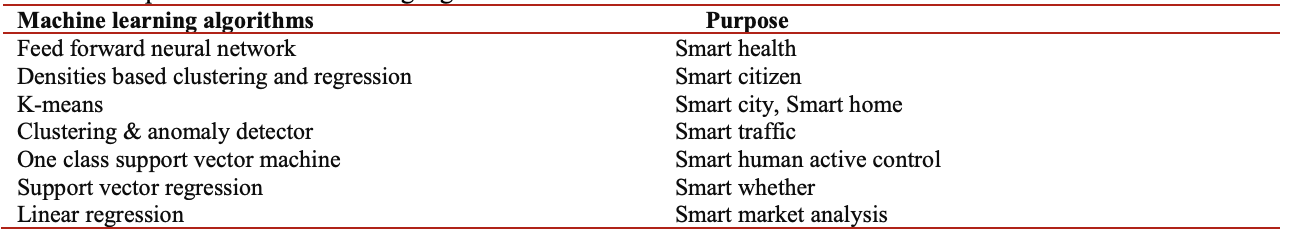
\includegraphics[width=1\textwidth]{ML_algorithms.png}
    \caption{Machine Learning Algorithms for specific applications \cite{Mohapatra}}
    \label{fig:applic}
\end{figure}

The bias-variance trade-off should be considered when optimising ML models. 
Bias is the model’s ability to learn the wrong things due to oversimplification or incorrect assumptions. 
Variance is the error due to sensitivity as a result of small fluctuations in training data. 
As the complexity of the model increases, bias decreases but the variance will increase. 
This is the trade-off between these two factors. 
An overfit model is one that is too complex resulting in high variance and low bias, while an underfit model has low variance and high bias due to its simplistic nature. 
Both overfit and underfit models are undesirable and it is ideal to find a suitable trade-off between bias and variance (hence complexity) to yield a well fit model capable of adapting to different datasets \cite{Jedamski}. 

\begin{figure}[H]
    \centering
    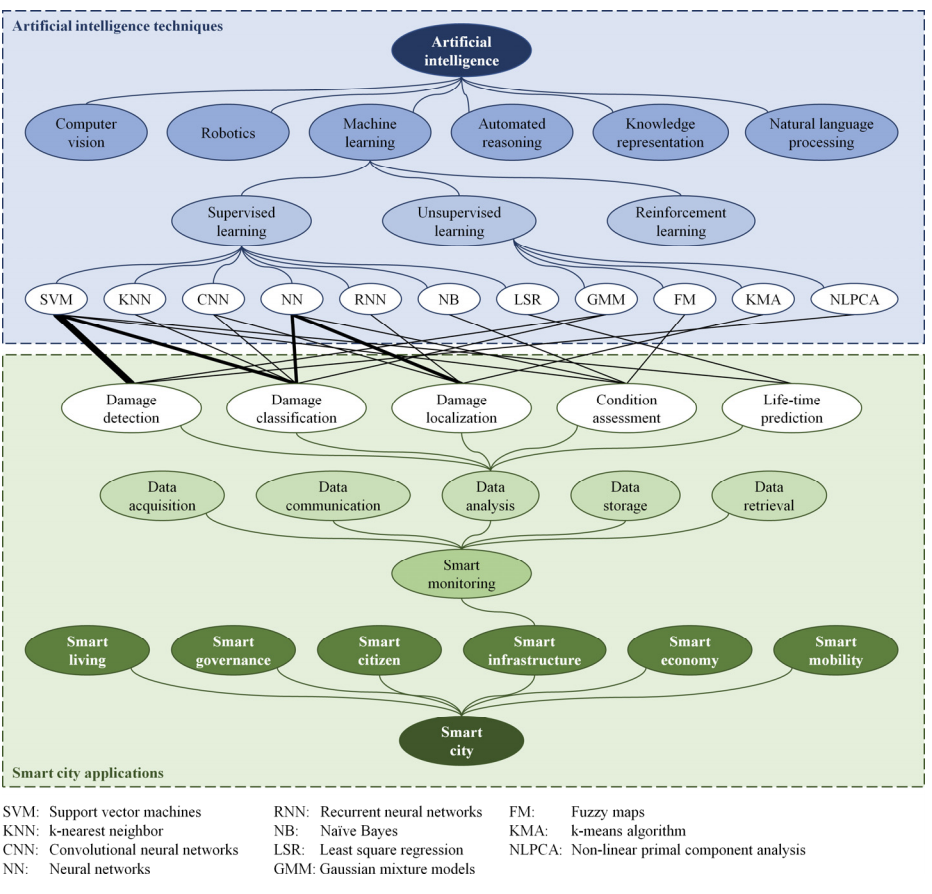
\includegraphics[width=\textwidth]{smart_monitoring_algorithms.png}
    \caption{Available ML algorithms for smart monitoring \cite{inproceedings}}
    \label{fig:algor}
\end{figure}

\enlargethispage{\baselineskip}
The dataset/s to be used in the above experiments will be obtained through various open-source data collections available online. 
Therefore, data collection is not a part of this project.
To ensure validity during the training of models, the data distribution will be split into three smaller datasets for training, validation and testing. 
The training set is used to train the models to fit the data and are evaluated against the validations set. 
The validation set being unseen, allows us to determine which models are generalising well to new examples. 
After the best model has been selected it is again tested on the test dataset as a final check on its generalisation ability. 
The training set accounts for 60\% of the full data set, while the validation and test sets account for 20\% each. 

\section{Reward Hacking}
The two unreliability factors discussed in the above experiments are concerned mainly with supervised learning models. 
A major reliability issue within reinforcement learning models is reward hacking. 
We will perform a systematic literature review on applications and known causes of unreliability due to reward hacking as well as potential solutions.

%% Label Bias and Environmental Datashift
\chapter{Label Bias and Environmental Datashift}
Bias is the result of inadequate data where a certain group or class is favoured over another/others hence creating an overrepresentation \cite{Jiang}\cite{saria2019tutorial}.
ML models trained using such datasets will acquire these underlying biases hence making incorrect predictions.

The following mathematical framework can be used as a representation to undestand bias in data \cite{Jiang}

\begin{figure}[h]
    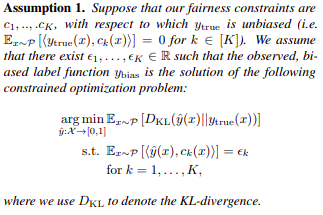
\includegraphics[scale =0.8]{Assumption.png}
    \centering
    \caption{Bias Assumption \cite{Jiang}}
    \label{fig:Assumption}
\end{figure}

In figure \ref{fig:Assumption}, the assumption is that $y_{bias}$ is the label which is closest to $y_{true}$ and achieves the same amount of bias.
In cases where data has been manually manipulated by humans, either consciously or subconsciously, this is deemed to be a reasonable assumption.
The contiguity to $y_{true}$ is given by the KL-divergance, which is used to establish the notion of accurate labeling. 
The Proposition in figure \ref{fig:Proposition} is derived from the KL-divergence. (For complete proof of proposition, see \cite{Jiang})

\begin{figure}[h]
    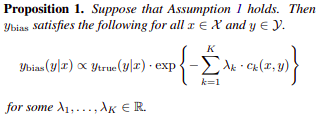
\includegraphics[scale =0.8]{Prop.png}
    \centering
    \caption{Bias Proposition \cite{Jiang}}
    \label{fig:Proposition}
\end{figure}

Now that $y_{bias}$ is represented in terms of $y_{true}$, we can infer $y_{true}$ in terms of $y_{bias}$ as represented in Figure \ref{fig:Corollary}.

\begin{figure}[h]
    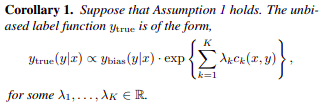
\includegraphics[scale =0.8]{corollary.png}
    \centering
    \caption{Bias Corollary \cite{Jiang}}
    \label{fig:Corollary}
\end{figure}

There may be situations where performance issues may not be apparent during training stages. 
They instead appear post-deployment where training and deployment datasets can have irregularities. 
This is known as Environmental Datashift. This calls into question whether the ML model is robust enough to generalise well to new samples beyond training, or whether it tends to over-generalise to the training dataset.


\section{Dataset \& Preprocessing}
The predictive maintenance dataset will be used again to classify failures of an ioT gadget.
During one week, maintenance data was collected from six devices every hour for 168 hrs.
Therefore, this data set contains 1008 rows of data. 
Each cycle of data reading contains the following measurements: 

%% Suitable Algorithm Selection
\chapter{Suitable Algorithm Selection}
\section{Dataset \& Preprocessing}
The predictive maintenance dataset will be used again to classify failures of an ioT gadget.
During one week, maintenance data was collected from six devices every hour for 168 hrs.
Therefore, this data set contains 1008 rows of data. 
Each cycle of data reading contains the following measurements: 

\begin{table}[ht]
    \begin{center}
        \caption{Measurements Dataset} 
        \begin{tabular}{ l|l } 
         \hline
         \textbf{Measurement} & \textbf{Description} \\  [0.5ex] 
         \hline
         \textbf{Measurement Time} & Time \\
         \textbf{Gadget ID} & Device number \\
         \textbf{Vibration x sensor} & Horizontal vibration \\ 
         \textbf{Vibration y sensor} & Vertical vibration \\ 
         \textbf{pressure sensor} & Hose pressure \\
         \textbf{Temperature sensor} & Internal temperature \\
         \hline
        \end{tabular}
    \end{center}
\end{table}

The failures dataset contains the precise times each gadget failed. 
During the course of the week, 105 failures were recorded.
Device failure is to be classified when the time remaining to device failure is less than one hour.

This dataset has been split into two datasets for training and testing respectively.
The training dataset will compromise of all data collected from gadget IDs 1-4, leaving data from gadgets 5 and 6 for the test set.
This will ensure the trained models are tested on completely new data. 

For more information on the dataset and use case, please see []
\hyperlink{gitub repo}{https://github.com/Unikie/predictive-maintenance-tutorial}

\section{Algorithms}
\subsection{Support Vector Machines}
Support Vector Machines (SVM) is a common supervised machine learning algorithm for both classification and regression tasks.
A key attribute of SVMs is its high accuracy and precision in thge segregation of classes.
SVMs create $n$-dimensional hyperplanes to segregate datapoints into $n$ number of classes/groups. 
The algorithm aims to achieve the maximum margin between support vecotrs(closest points), i.e. maximise the minimum margin.

In the case where two classes can be linearly seperated, we consider the following as a representation of a dataset, $S$.
\begin{equation}
    S = \Big\{x_i \in \R^{1 \times p}, y_i \in \{-1, 1\}\Big\}^n_{i=1}
\end{equation}

The values $\{-1, 1\}$ represent two classes of data, $A$ and $B$,
\begin{equation}
    y_i = \begin{cases}
        1, & \text{if $i$} \text{-th sample} \in  A\\
        -1, & \text{if $i$} \text{-th sample} \in  B.
    \end{cases}
\end{equation}

The hyperplane can then be defined as $F_0$ in $\R^D$ space as,
\begin{equation}
    F_0 = \big \{x|f(x) = x \beta + \beta_0 = 0 \big \} 
\end{equation}  
where, 
$\beta \in \R^D$ with norm $||\beta|| = 1$

For a new sample $x^{new}$ which is not within dataset $S$, we can detemine a classification as,
\begin{equation}
    y_{new} = \begin{cases}
        1 \text{(Class A) }, & \text{if } f(x^{new}) > 0 \\
        -1 \text{(Class B) }, & \text{if } f(x^{new}) < 0
    \end{cases}
\end{equation}

%ref
% https://ieeexplore-ieee-org.ezproxy.lib.uts.edu.au/stamp/stamp.jsp?tp=&arnumber=6653952&tag=1
% https://pureadmin.qub.ac.uk/ws/files/17844756/machine.pdf


\subsection{k-Nearest Neighbours}
k-Nearst Neighbours (k-NN) is a simple supervised machine learning algorithm used in both classification and regression problems. 
This approach classifies objects based on the compuatational distances or similarities between samples/values.
The k-NN algorithm only requires tuning of a single parameter, $k$, which represents the amount of nearest samples within the neighbourhood.
The choice of $k$ will affect the algorithm's performance where a value too small would create higher variance hence resulting in less stability.
A larger $k$ value will produce higher bias resulting in lower precision. 

After the number of neighbours, $k$, has been selected, the distances between the query data point, $x_q$, and an arbitrary data point, $x_i$ are to be determined.
Most commonly used is the Euclidean distance (\ref{Euclidean}), however Manhattan distance (\ref{Manhattan}) may also be applied.

\begin{equation} \label{Euclidean}
    d(x_q,x_i) = \sqrt{\sum_{i=1}^{m} (x_q - x_i)^2}
\end{equation}
\begin{equation} \label{Manhattan}
    d(x_q,x_i) = \sum_{i=1}^{m} \lvert x_r - x_i \rvert
\end{equation}

The resulting values are then sorted by distance from smallest to largest and the first $k$ entries are selected. 
In classification problems, the mode of $k$ labels is returned, while the mean of $k$ labels is returned in regression problems.

% references:
% https://towardsdatascience.com/machine-learning-basics-with-the-k-nearest-neighbors-algorithm-6a6e71d01761
% https://www.listendata.com/2017/12/k-nearest-neighbor-step-by-step-tutorial.html
% http://www.lkozma.net/knn2.pdf
% https://ieeexplore-ieee-org.ezproxy.lib.uts.edu.au/stamp/stamp.jsp?tp=&arnumber=7456223

\subsection{Random Forest}
Random Forest is an ensemble machine learning method which creates multiple random decision trees and combines their respective votes (classification) or averages (regression) to improve prediction accuracy and fitting.

\enlargethispage{3\baselineskip}
\begin{figure}[h]
    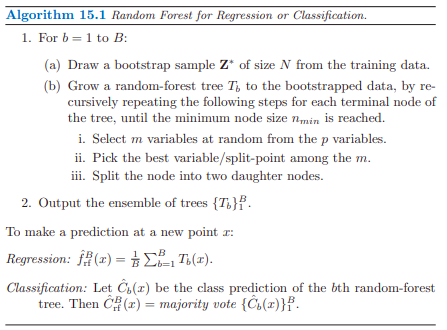
\includegraphics[scale=0.7]{random_forest.png}
    \centering
    % \caption{Random Forest Algorithm \cite{chen}}
    \label{fig:RF}
\end{figure}

% Ref:
% https://www.math.mcgill.ca/yyang/resources/doc/randomforest.pdf

\subsection{Neural Networks}

\section{Results}
\section{Recommendations}
Literature review:

Regression application - Prediction of Remaining Useful Lifetime (RUL) of
Turbofan Engine using Machine Learning 

%% Reward Hacking
\chapter{Reward Hacking}

%% Conclusion
\chapter{Conclusion}

%% Bibliography
\renewcommand{\bibname}{References}
\bibliographystyle{ieeetr}
\bibliography{references}

\end{document}